\documentclass[12pt,openany]{book}

\usepackage{amsmath,amsthm,amsfonts,amscd} % Packages for mathematics

% Colors
\usepackage[dvipsnames, table]{xcolor}
\definecolor{titleblue}{RGB}{0,53,128}
\definecolor{chaptergray}{RGB}{140,140,140}
\definecolor{sectiongray}{RGB}{180,180,180}

\definecolor{thmcolor}{RGB}{231, 76, 60}
\definecolor{defcolor}{RGB}{52, 152, 219}
\definecolor{lemcolor}{RGB}{155, 89, 182}
\definecolor{corcolor}{RGB}{46, 204, 113}
\definecolor{procolor}{RGB}{241, 196, 15}

% Fonts
\usepackage[T1]{fontenc}
\usepackage[utf8]{inputenc}
\usepackage{newpxtext,newpxmath}
\usepackage{sectsty}
\allsectionsfont{\sffamily\color{titleblue}\mdseries}

% Page layout
\usepackage{geometry}
\geometry{a4paper,left=1in,right=.7in,top=1in,bottom=1in,heightrounded}
\usepackage{fancyhdr}
\fancyhf{}
\fancyhead[LE,RO]{\thepage}
\fancyhead[LO]{\nouppercase{\rightmark}}
\fancyhead[RE]{\nouppercase{\leftmark}}
\renewcommand{\headrulewidth}{0.5pt}
\renewcommand{\footrulewidth}{0pt}

% Chapter formatting
\usepackage{titlesec}
\titleformat{\chapter}[display]
{\normalfont\sffamily\Huge\bfseries\color{titleblue}}{\chaptertitlename\ \thechapter}{20pt}{\Huge}
\titleformat{\section}
{\normalfont\sffamily\Large\bfseries\color{titleblue!100!gray}}{\thesection}{1em}{}
\titleformat{\subsection}
{\normalfont\sffamily\large\bfseries\color{titleblue!75!gray}}{\thesubsection}{1em}{}

% Table of contents formatting
\usepackage{tocloft}
\renewcommand{\cftchapfont}{\sffamily\color{titleblue}\bfseries}
\renewcommand{\cftsecfont}{\sffamily\color{chaptergray}}
\renewcommand{\cftsubsecfont}{\sffamily\color{sectiongray}}
\renewcommand{\cftchapleader}{\cftdotfill{\cftdotsep}}

% Hyperlinks
\usepackage{hyperref}
\hypersetup{
	colorlinks=true,
	linkcolor=titleblue,
	filecolor=black,      
	urlcolor=titleblue,
}

%Listing
\usepackage{listings} %Code
\renewcommand{\lstlistingname}{Code}%

\definecolor{sagegreen}{rgb}{0.0,0.6,0.4}
\definecolor{sagepurple}{rgb}{0.6,0.0,0.4}
\definecolor{sageblue}{rgb}{0.0,0.4,0.6}
\definecolor{sageorange}{rgb}{1.0,0.4,0.0}
\definecolor{sagegray}{rgb}{0.4,0.4,0.4}

\lstdefinestyle{sage}{
	language=Python,
	backgroundcolor=\color{white},
	basicstyle=\small\ttfamily\color{black}, 
	basicstyle=\footnotesize\ttfamily\color{black},
	keywordstyle=\color{blue!60!black},
	commentstyle=\color{green!60!black},
	stringstyle=\color{purple!60!black},
	showstringspaces=false,
	breaklines=true,
	tabsize=4,
	morekeywords={True, False, None},
	frame=leftline, % Remove the border
	framesep=3pt,
	frameround=tttt,
	framexleftmargin=3pt,
	numbers=left,
	numberstyle=\small\color{gray},
	xleftmargin=15pt, % Increase the left margin
	xrightmargin=5pt,
	captionpos=b,
	belowskip=0pt,
	aboveskip=4pt
}

%Ceiling and Floor Function
\usepackage{mathtools}
\DeclarePairedDelimiter{\ceil}{\lceil}{\rceil}
\DeclarePairedDelimiter{\floor}{\lfloor}{\rfloor}

%Algorithm
\usepackage[ruled,linesnumbered]{algorithm2e}
\usepackage{setspace}
\usepackage{algpseudocode}
\SetKwComment{Comment}{/* }{ */}
\SetKw{Break}{break}
\SetKw{Downto}{downto}
\SetKwProg{Fn}{Function}{:}{end}
\SetKwFunction{KeyGens}{KeyGens}

\renewcommand{\arraystretch}{1.25}
%---------------------------My Preamble
\usepackage{marvosym} %Lightning
\usepackage{booktabs}
\usepackage{multicol}
\setlength{\columnsep}{2cm}
\setlength{\columnseprule}{1.25pt}
\usepackage{enumerate}
\usepackage{soul}
\newcommand{\mathcolorbox}[2]{\colorbox{#1}{$\displaystyle #2$}}
\usepackage{graphicx}
\usepackage{tikz}
\usepackage{tikz-cd}
\usetikzlibrary{calc}
\usetikzlibrary{arrows, arrows.meta, positioning, shapes.multipart}

%Tcolorbox
\usepackage[most]{tcolorbox}
\tcbset{colback=white, arc=5pt}
%\tcbset{enhanced, colback=white,colframe=black,fonttitle=\bfseries,arc=4mm,boxrule=1pt,shadow={2mm}{-1mm}{0mm}{black!50}}
%White box with black text and shadow
%\begin{tcolorbox}[colback=white,colframe=black,fonttitle=\bfseries,title=Black Shadow Box,arc=4mm,boxrule=1pt,shadow={2mm}{-1mm}{0mm}{black!50}]
%	This is a white box with black text and a subtle shadow. The shadow adds some depth and dimension to the box without overpowering the design.
%\end{tcolorbox}

%Theorem
\newtheorem{axiom}{Axiom}[chapter]
\newtheorem{theorem}{Theorem}[chapter]
\newtheorem{proposition}[theorem]{Proposition}
\newtheorem{corollary}{Corollary}[theorem]
\newtheorem{lemma}[theorem]{Lemma}

\theoremstyle{definition}
\newtheorem{definition}{Definition}[chapter]
\newtheorem{construction}{Construction}[chapter]
\newtheorem{remark}{Remark}[chapter]
\newtheorem{exercise}{Exercise}[chapter]
\newtheorem{example}{Example}[chapter]
\newtheorem*{note}{Note}

%New Command
\newcommand{\set}[1]{\left\{#1\right\}}
\newcommand{\N}{\mathbb{N}}
\newcommand{\Z}{\mathbb{Z}}
\newcommand{\Q}{\mathbb{Q}}
\newcommand{\R}{\mathbb{R}}
\newcommand{\C}{\mathbb{C}}
\newcommand{\F}{\mathbb{F}}

\newcommand{\inv}[1]{#1^{-1}}

\newcommand{\ie}{\textnormal{i.e.}}
\newcommand{\eg}{\textnormal{e.g.}}

\newcommand{\of}[1]{\left( #1 \right)} 
\newcommand{\abs}[1]{\left\lvert #1 \right\rvert}
\newcommand{\norm}[1]{\left\| #1 \right\|}

\newcommand{\KeyGen}{\mathsf{KeyGen}}
\newcommand{\Enc}{\mathsf{Enc}}
\newcommand{\Dec}{\mathsf{Dec}}
\newcommand{\scheme}{\Sigma}
\newcommand{\keyspace}{\mathcal{K}}
\newcommand{\messagespace}{\mathcal{M}}
\newcommand{\ciphertextspace}{\mathcal{C}}

\newcommand{\library}{\mathcal{L}}
\newcommand{\zero}{\textcolor{red}{\texttt{0}}}
\newcommand{\one}{\textcolor{red}{\texttt{1}}}

\newcommand{\tab}{\hspace{8pt}}
\newcommand{\xor}{\oplus}
\newcommand{\adversary}{\mathcal{A}}
\newcommand{\isequal}{\overset{?}{=}}
\newcommand{\linking}{\diamond}

\newcommand{\true}{\texttt{true}}
\newcommand{\false}{\texttt{false}}
\newcommand{\randomness}{\$}
\newcommand{\uniform}{\xleftarrow{\randomness}}
\newcommand{\binaryfield}{\set{\zero,\one}}

\newcommand{\ctxt}{\texttt{CTXT}}
\newcommand{\eavesdrop}{\texttt{Eavesdrop}}

% Begin document
\begin{document}
	
	% Title page
	\begin{titlepage}
		\begin{center}
			{\Huge\textsf{\textbf{Code-Based Games Philosophy}}\par}
			\vspace{0.5in}
			{\Large Ji Yong-Hyeon, Kim Dong-Hyeon\par}
			\vspace{1in}
			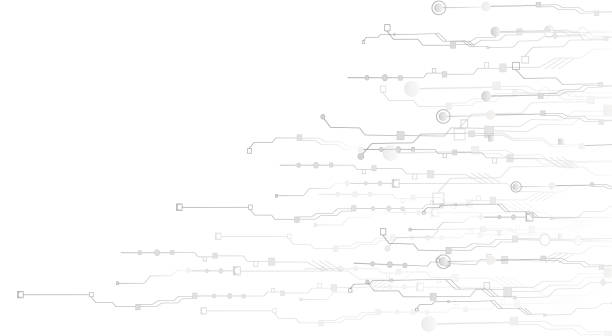
\includegraphics[scale=2.5]{urop.jpg}\par
			\vspace{1in}
			{\bf Department of Information Security, Cryptology, and Mathematics\par}
			{College of Science and Technology\par}
			{Kookmin University\par}
			%
\includegraphics[width=1.5in]{school_logo.jpg}\par
			\vspace{.25in}
			{\large \today\par}
		\end{center}
	\end{titlepage}
	
	% Table of contents
	\tableofcontents
	
	% Chapters
	\mainmatter
	
	\chapter*{List of Symbols}
	
	\begin{tabular}{ll}
		\( \zero^\lambda, \one^\lambda\) & \(\underbrace{\zero\zero\cdots\zero}_{\lambda\ \text{times}}, \underbrace{\one\one\cdots\one}_{\lambda\ \text{times}}\) : \(\lambda\)-bit zero/one sequence \\
		\( \adversary\linking\library \) & The result of \textbf{linking} $\adversary$ to  $\library$ \\
		\( \randomness \) & Randomeness \\
	\end{tabular}
	
	\chapter{One-Time Pad \& Kerckhoff's Principle}
	
	\begin{tcolorbox}[colback=white,colframe=gray,arc=5pt,title={\color{white}\bf }]
		\textbf{Kerchkhoffs' Principle:}
		\begin{quote}
			Design your system to be secure even if the attacker has complete knowledge of all its algorithms.
		\end{quote}
	\end{tcolorbox}
	\vspace{8pt}
	\begin{tcolorbox}[colback=white,colframe=defcolor,arc=5pt,title={\color{white}\bf One-time Pad (OTP)}]
		\begin{construction}
			The specific \(\KeyGen,\Enc\), and \(\Dec\) algorithms for \textbf{one-time pad} are given below: \begin{center}
				\begin{tabular}{|lll|}
					\hline
					$\underline{\KeyGen:}$ & \(\underline{\Enc(k,m\in\binaryfield^\lambda):}\) & \(\underline{\Dec(k,c\in\binaryfield^\lambda):}\)\\
					\tab$k\uniform\binaryfield^\lambda$ & \tab return \(k\xor m\) & \tab return \(k\xor c\)\\
					\tab return $k$ &&\\
					\hline
				\end{tabular}\\
			\end{center}
		\end{construction}
	\end{tcolorbox}
	\vspace{8pt}
	\begin{tcolorbox}[colback=white,colframe=procolor,arc=5pt,title={\color{white}\bf Corectness of OTP}]
		\begin{proposition}
			\[
			(\forall k,m\in\binaryfield^\lambda)\quad\Dec(k,\Enc(k,m))=m.
			\]
		\end{proposition}
	\end{tcolorbox}
	\begin{proof}
		Let \(k,m\in\binaryfield^\lambda\) then \begin{align*}
			\Dec(k,\Enc(k,m))=\Dec(k,k\xor m)&=k\xor(k\xor m)\\
			&=(k\xor k)\xor m\\
			&=\zero^\lambda\xor m\\
			&=m.
		\end{align*}
	\end{proof}

	\newpage
	\begin{remark}[\eavesdrop\ Algorithm]
		From Eve’s perspective, seeing a ciphertext corresponds to receiving
		an output from the following algorithm: \\ \begin{center}
		\begin{tabular}{|l|}
			\hline
			\(\underline{\eavesdrop(m\in\binaryfield^\lambda)}\)\\
			\tab\(k\uniform\binaryfield^\lambda\)\\
			\tab\(c:=k\xor m\)\\
			\tab return \(c\)\\
			\hline
		\end{tabular}
		\end{center}
	\end{remark}

	\begin{tcolorbox}[colback=white,colframe=thmcolor,arc=5pt,title={\color{white}\bf }]
		\begin{theorem}
			Let \(m\in\binaryfield^\lambda\). The distribution \(\eavesdrop(m)\) is the \textbf{uniform distribution} on \(\binaryfield^\lambda\). In other words, \[
			m,m'\in\binaryfield^\lambda\implies\textnormal{dist}(\eavesdrop(m))\sim\textnormal{dist}(\eavesdrop(m')).
			\]
		\end{theorem}
	\end{tcolorbox}
	\begin{proof}
		content...
	\end{proof}
	
	\chapter{The Basics of Provable Security}
	
	\section{How to Write a Security Definition}
	\subsection{Syntax and Correctness}
	
	\begin{tcolorbox}[colback=white,colframe=defcolor,arc=5pt,title={\color{white}\bf Encryption Syntax}]
		\begin{definition}
			A \textbf{symmetric-key encryption (SKE) scheme} consists of the following algorithms: \begin{itemize}
				\item $\KeyGen$ outputs a key $k=\KeyGen(1^\lambda)\in\keyspace$
				\item $\Enc:\keyspace\times\messagespace\to\ciphertextspace$
				\item $\Dec:\keyspace\times\ciphertextspace\to\messagespace$
			\end{itemize} We call $\keyspace$ the \textbf{key space}, $\messagespace$ the \textbf{message space}, and $\ciphertextspace$ the \textbf{ciphertext space} of the scheme.
		\end{definition}
	\end{tcolorbox}
	\begin{remark}
		Note that \begin{itemize}
			\item \(\KeyGen\) is a randomized algorithm\footnote{An algorithm that makes use of random numbers.}.
			\item \(\Enc\) is a (possibly randomized) algorithm\footnote{It could operate deterministically or non-deterministically depending on specific conditions or parameters.}.
			\item \(\Dec\) is a deterministic algorithm\footnote{An algorithm that does produces the same output for the same input, every time it's run.}.
		\end{itemize}
	\end{remark}
	\begin{remark}
		We refer to the entire scheme by a single variable $\scheme$, \ie, $$
		\scheme=(\KeyGen, \Enc, \Dec).
		$$
	\end{remark}
	\begin{remark}
		We write \[
		\begin{array}{ccc}
			\scheme.\KeyGen, & \scheme.\Enc, & \scheme.\Dec,\\
			\scheme.\keyspace, & \scheme.\messagespace, &\scheme.\ciphertextspace
		\end{array}
		\] to refer to its components.
	\end{remark}
	\vspace{8pt}
	\begin{tcolorbox}[colback=white,colframe=defcolor,arc=5pt,title={\color{white}\bf SKE Correctness}]
		\begin{definition}
			An encryption scheme $\scheme$ satisfies \textbf{correctness} if \[
			\left(\forall k\in\scheme.\keyspace\right)\left(\forall m\in\scheme.\messagespace
			\right)\quad\Pr\left[\scheme.\Dec(k, \scheme.\Enc(k,m))=m\right]=1.
			\]
		\end{definition}
	\end{tcolorbox}
	\begin{remark}
		The definition is written in terms of a probability because $\Enc$ is allowed to be a randomized algorithm. In other words, decrypting a ciphertext with the same key that was used for encryption must \textit{always} result in the original plaintext.
	\end{remark}
	\vspace{4pt}
	\begin{example}
		content...
	\end{example}
	
	\subsection{``Real-vs-Random'' Style of Security Definition}
	\begin{quote}
		``an encryption scheme is a good one if its ciphertexts \textit{look like} random junk to an attacker''
	\end{quote}

	Security definitions always consider \textbf{the attacker's view} of the system.
	\begin{quote}
		``an encryption scheme is a good one if its ciphertexts \textit{look like} random junk to an attacker ... when each key is secret and used to encrypt only one plaintext, even when the attacker chooses the plaintexts.''
	\end{quote}

	
	A concise way to express all of these details is to consider \textbf{the attacker as a calling	program} to the following subroutine:
	\begin{center}
		\begin{tabular}{|l|}
			\hline
			$\underline{\texttt{CTXT}(m\in\scheme.\messagespace):}$\\
			\tab$k\gets\scheme.\KeyGen$\\
			\tab$c:=\scheme.\Enc(k,m)$\\
			\tab return $c$\\
			\hline
		\end{tabular}\\
	\end{center}
	
	\begin{example}[One-Time Pad (OTP)]
		a\\ \begin{center}
			\begin{minipage}{.44\textwidth}
				\begin{tabular}{|l|}
					\hline
					$\underline{\texttt{CTXT}(m):}$\\
					\begin{tabular}{ll}
						\tab$k\gets\binaryfield^\lambda$ & \textcolor{gray}{//\(\KeyGen\) of OTP}\\
						\tab$c:=k\xor m$ & \textcolor{gray}{//\(\Enc\) of OTP}\\
						\tab return $c$\\
					\end{tabular}\\
					\hline
				\end{tabular}\\
			\end{minipage} vs.
		\begin{minipage}{.3\textwidth}
			\begin{tabular}{|l|}
				\hline
				$\underline{\texttt{CTXT}(m):}$\\
				\begin{tabular}{ll}
					\tab$c:=\binaryfield^\lambda$ & \textcolor{gray}{//\(\ciphertextspace\) of OTP}\\
					\tab return $c$\\
				\end{tabular}\\
				\hline
			\end{tabular}\\
		\end{minipage}
		\end{center}
	\end{example}

	\begin{quote}
		``an encryption scheme is a good one if, when you plug its \(\KeyGen\) and \(\Enc\) algorithms into the template of the \texttt{CTXT} subroutine above, the two implementations of \texttt{CTXT} induce identical behavior in every calling program.''
	\end{quote}

	\subsection{``Left-vs-Right'' Style of Security Definition}
	
	\section{Formalisms for Security Definition}
	\begin{tcolorbox}[colback=white,colframe=defcolor,arc=5pt,title={\color{white}\bf Library}]
		\begin{definition}
			A \textbf{library} $\library$ is a collection of subroutines and private/static variables.
		\end{definition}
	\end{tcolorbox}
	\begin{example}
		Here is a familiar library and one possible calling program:
		\begin{center}
			\begin{minipage}{.25\textwidth}
				\begin{tabular}{|c|}
					\hline
					\cellcolor{blue!25}$\library$\\
					\hline
					\begin{tabular}{l}
						\underline{\texttt{CTXT}($m$):}\\
						\tab $k\gets\set{\zero, \one}^\lambda$\\
						\tab $c:=k\xor m$\\
						\tab return $c$
					\end{tabular}\\
					\hline
				\end{tabular}\quad,\quad
			\end{minipage}
			\begin{minipage}{.25\textwidth}
				\begin{tabular}{|c|}
					\hline
					\cellcolor{blue!25}$\adversary$\\
					\hline
					\begin{tabular}{l}
						$m\gets\set{\zero,\one}^\lambda$\\
						$c:=\texttt{CTXT}(m)$\\
						return $m\isequal c$
					\end{tabular}\\
					\hline
				\end{tabular}
			\end{minipage}.
		\end{center} Then \[
		\Pr\left[\adversary\linking\library\Rightarrow\true\right]=\frac{1}{2^\lambda}.
		\]
	\end{example}
	\vspace{8pt}
	\begin{tcolorbox}[colback=white,colframe=defcolor,arc=5pt,title={\color{white}\bf Interchangeability}]
		\begin{definition}
			Let $\library_1$ and $\library_2$ be two libraries that have the same interface. We say that $\library_1$ and $\library_2$ are \textbf{interchangeable}, and write $\library_1\equiv\library_2$, if $\forall\adversary:$\[
			\Pr\left[\adversary\linking\library_1\Rightarrow\true\right]=
			\Pr\left[\adversary\linking\library_2\Rightarrow\true\right].
			\]
		\end{definition}
	\end{tcolorbox}
	\vspace{8pt}

	\begin{tcolorbox}[colback=white,colframe=defcolor,arc=5pt,title={\color{white}\bf One-Time Uniform Ctxts}]
		\begin{definition}
			An encryption scheme $\scheme$ has \textbf{one-time uniform cipher-texts} if 
			\begin{center}
				\begin{minipage}{.3\textwidth}
					\begin{tabular}{|c|}
						\hline
						\cellcolor{blue!25}$\library_{\text{ots\$-real}}^\scheme$\\
						\hline
						\begin{tabular}{l}
							\underline{\texttt{CTXT}($m\in\scheme.\messagespace$):}\\
							\tab $k\gets\scheme.\KeyGen$\\
							\tab $c\gets\scheme.\Enc(k,m)$\\
							\tab return $c$
						\end{tabular}\\
						\hline
					\end{tabular}
				\end{minipage}
				$\equiv$\quad
				\begin{minipage}{.3\textwidth}
					\begin{tabular}{|c|}
						\hline
						\cellcolor{blue!25}$\library_{\text{ots\$-rand}}^\scheme$\\
						\hline
						\begin{tabular}{l}
							\underline{\texttt{CTXT}($m\in\scheme.\messagespace$)}:\\
							\tab $c\gets\scheme.\ciphertextspace$\\
							\tab return $c$
						\end{tabular}\\
						\hline
					\end{tabular}
				\end{minipage}
			\end{center}
		\end{definition}
	\end{tcolorbox}
	
	\section{How to Demonstrate Insecurity with Attacks}
	\section{How to Prove Security with The Hybrid Technique}
	\section{How to Compare/Contract Security Definitions}
	
	\newpage
	\chapter{Basing Cryptography on Intractable Computations}
	
	% End document
\end{document}
